\section{Architecture}
\label{sec:arch}

This section presents the architecture and design decisions taken to
create the \sdr platform. At the heart of our design are three main
points: \emph{low-power}, \emph{small size}, and \emph{low cost}. We
relax the modular design of existing SDR systems to reduce size and
cost, while promoting the FPGA to a first class citizen.

As discussed previously, a fast interconnect is essential to achieve
low radio latencies which today's radio standards require. We have to
use a fast, but low-power interconnect between the FPGA and the
processing core to achieve this. One possibility is to use an external
memory interface existing on many low-power microcontrollers to
connect to the FPGA. While this allows for a flexible choice of
microcontroller and FPGA, it has the disadvantage of greater physical
space requirements, limited bandwidth due to a limited bus data width,
and potentially increased costs due to additional chip packaging
needs.

ARM provides several options both on the low-power computing core and
bus architecture front. All major FPGA vendors sell system-on-chip
packages that contain high-speed ARM cores integrated with
leading-edge FPGAs. The cores and the FPGA are most often connected
through the AMBA High-performance Bus (AHB). The AHB is a pipelined,
single clock-edge on-chip bus to connect peripherals, memories, and
cores on a system-on-chip and provides a bandwidth of up to
16~GBit/s. An even faster version of the AHB is the Advanced
eXtensible Interface (AXI) which is used in Xilinx's Zynq
reconfigurable SoC that marries a dual-core ARM Cortex-A9 with a
Xilinx FPGA in one package \cite{zynq}. Altera has a similar SoC
combining a dual-core ARM Cortex-A9 with their Arria V or Cyclone V
FPGA series. Altera's bus interface has a peak bandwidth of up to
100~GBit/s \cite{alteraSoC}. While these systems are very impressive
with respect to processing power and speed, their power draw is in the
multiple-Watts range, which is outside of our goal for a low-power,
battery-operated solution.

\begin{figure}[t]
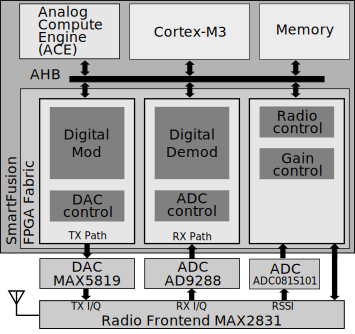
\includegraphics[width=0.98\columnwidth]{system_arch}
\caption{\sdr system architecture. The FPGA Fabric hosts the transmit,
receive, and radio control and is directly connected to the AMBA
High-performance Bus (AHB), together with the memory, analog compute engine
(ACE) and the ARM Cortex-M3 core. This rapid interface allows direct
memory-mapped access from the core to the SDR blocks. }
\label{fig:system_arch}
\end{figure}

\begin{figure}[th]
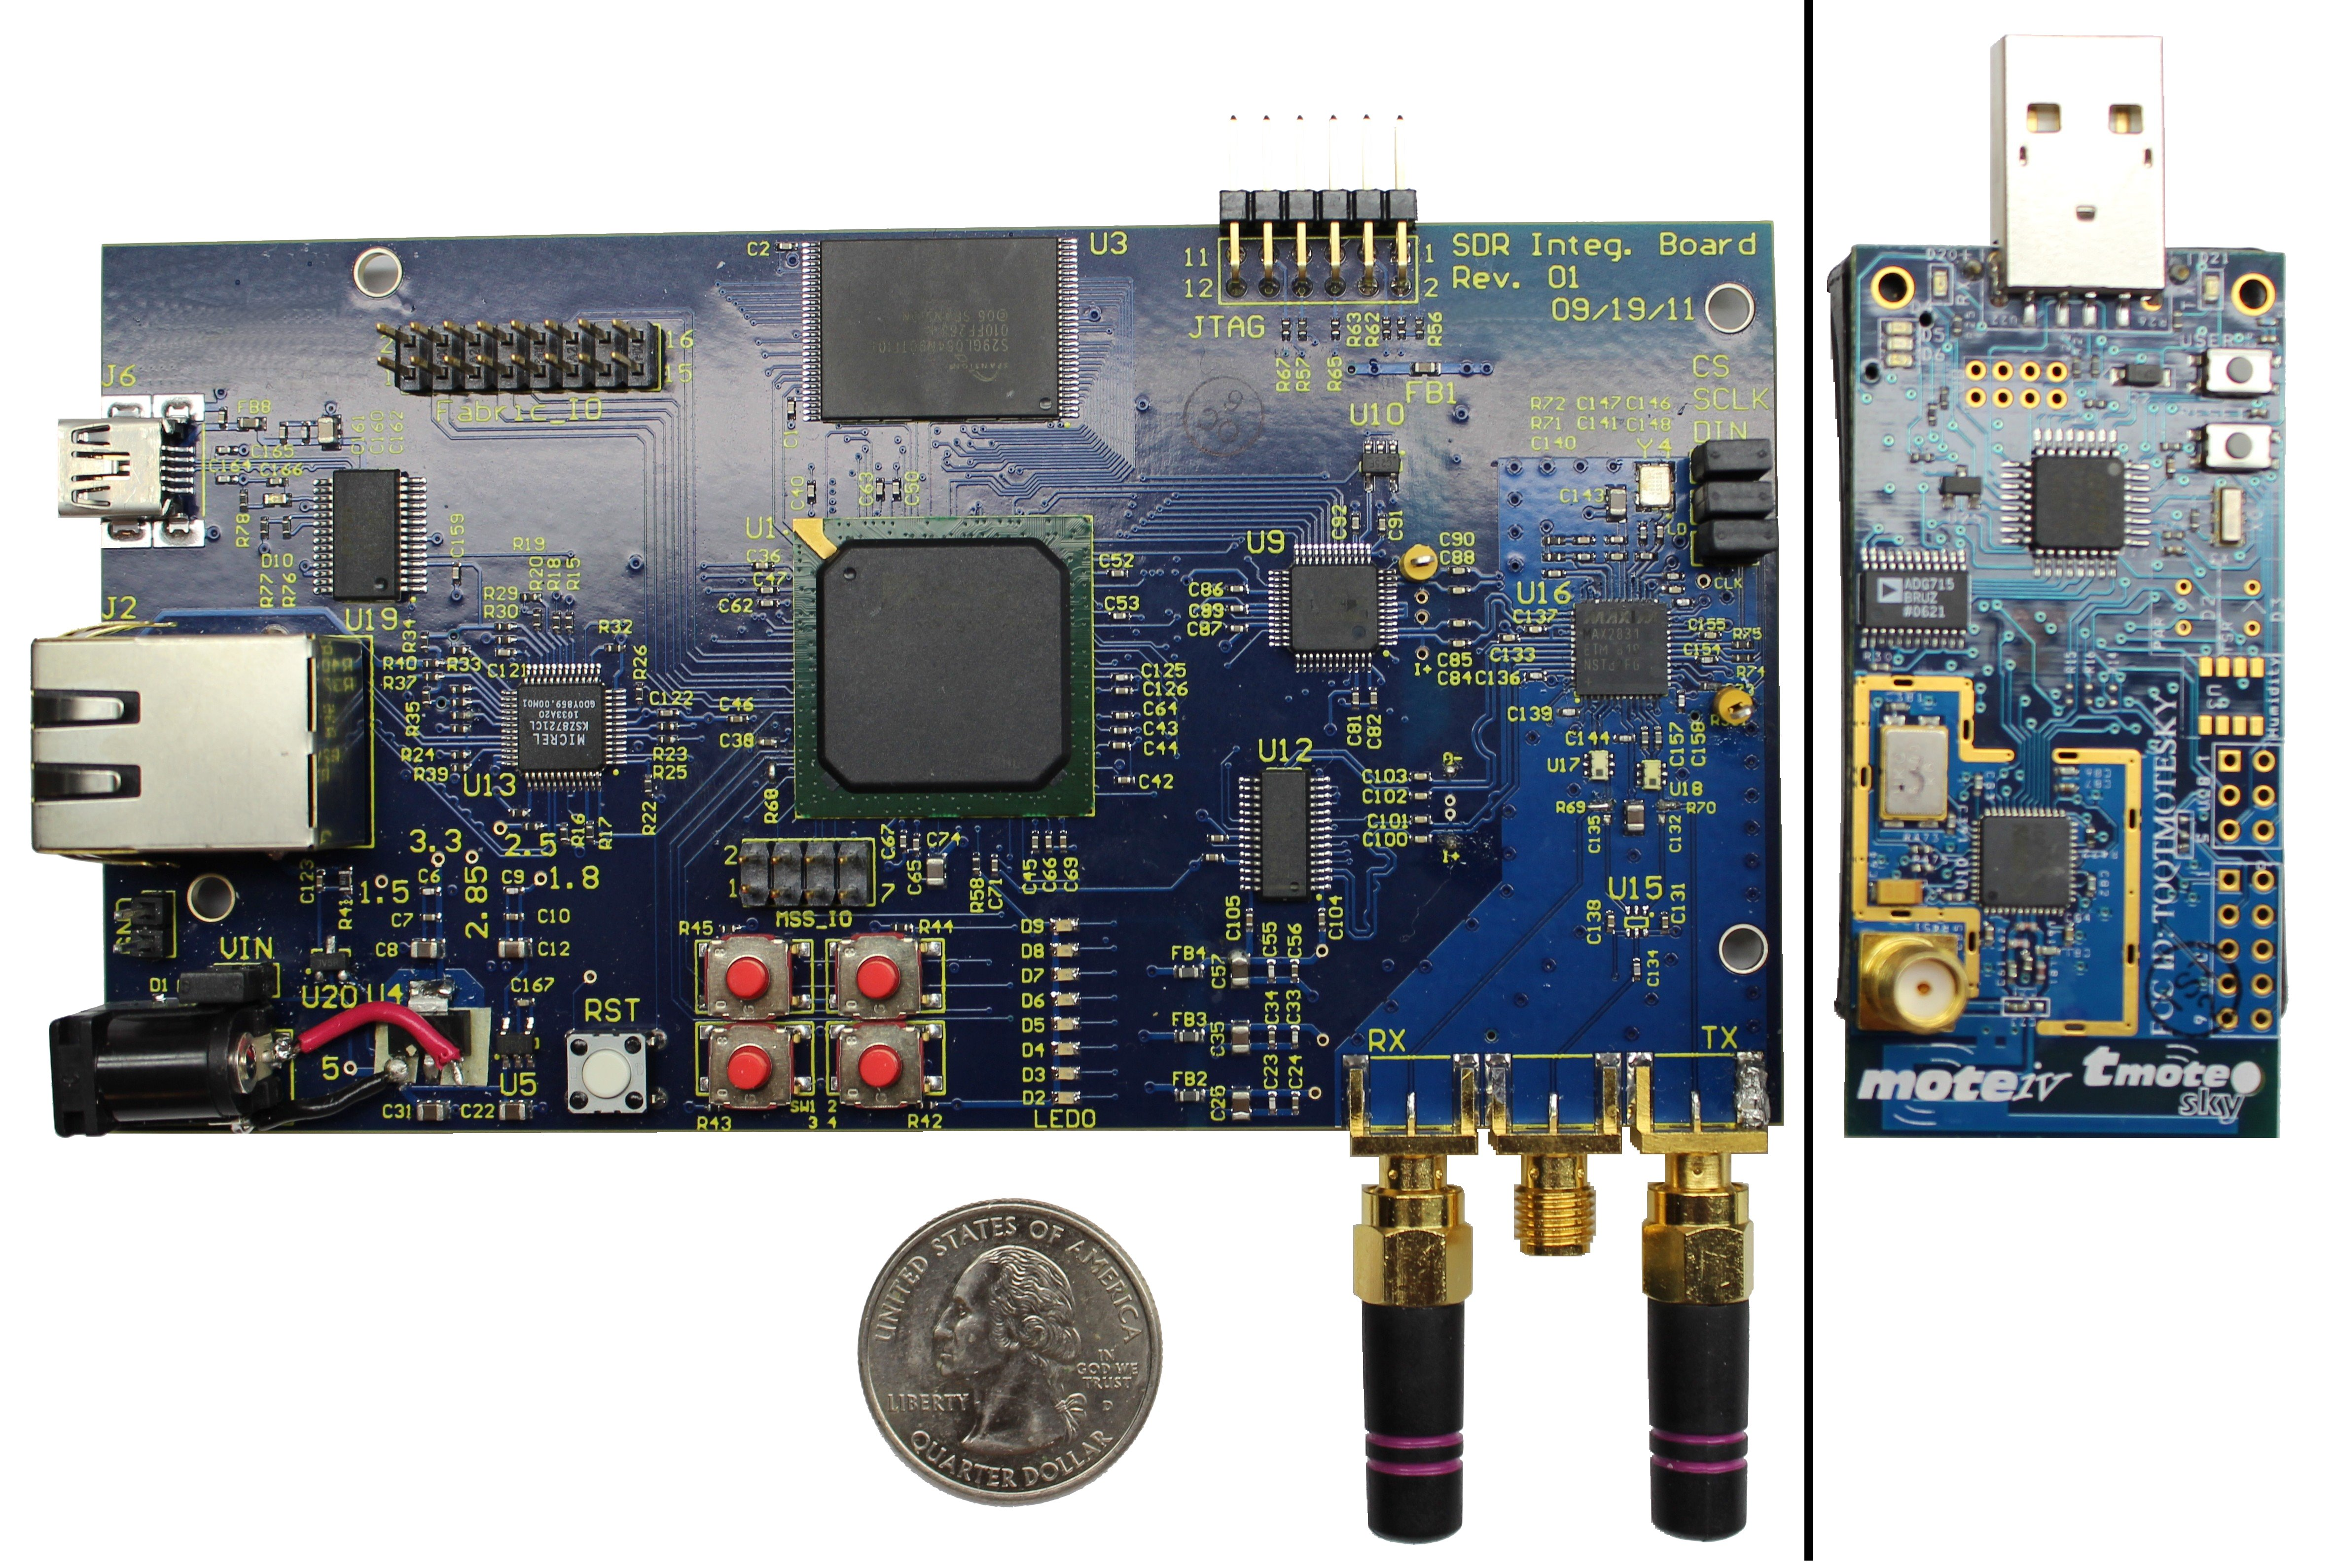
\includegraphics[width=0.98\columnwidth]{sdr_scale_tmote}
\caption{Picture of the \sdr platform. It measures 13~$\times$~7~cm and runs
for 7.5~hours without duty cycling from 4 AA batteries, allowing for the first
time true mobile SDR experiments. Shown for scaling is the TMote Sky. The
current \sdr is approximately four times the size of the Sky. Removing
extraneous inputs (Ethernet, etc) and debugging headers, \sdr is approximately
twice as large as the Sky.}
\label{fig:usdr}
\end{figure}

Microsemi, a vendor of flash-based FPGAs like the IGLOO series with
flash-freeze capabilities \cite{igloo} offers a third alternative in the
SmartFusion customizable System-on-Chip (cSoC). The SmartFusion contains an
ARM Cortex-M3 with a flash-based FPGA, connected through an AHB bus interface.
The flash-based FPGA brings the advantage of instant-on at power up, as the
configuration is stored in the FPGAs floating-gate memory. The AHB
interconnect allows a developer to write its own custom peripheral on the
FPGA, and access it through memory-mapped IO, as if it were a regular
peripheral. This allows for very fast and simple interaction between the
software and hardware side of the developed SDR code base, and a flexible
division between software-hardware boundary.

Beside the FPGA, the SmartFusion contains a rich set of standard
microcontroller peripherals (timers, serial bus interfaces, memories, etc) in
addition to an analog compute engine (ACE) with an ADC, DAC, and several
amplification and filtering options. By adding an RF radio frontend to the
ACE, the SmartFusion would be ready for SDR duties. However, at a maximum
speed of only $\sim$700~kS/s, the on-board ADC and DAC would limit us to low
data-rate communication.

We add an external high-speed ADC and DAC to the \sdr platform in order to
overcome the limits imposed by the ACE. Figure \ref{fig:system_arch} shows a
block diagram of the major components on the SmartFusion, as well as the
external ADC, DAC, and radio frontend chips. Figure \ref{fig:usdr} shows a
picture of the actual platform. The SmartFusion (U1) is the largest chip, located
at the center of the PCB. The ADC (U9) and DAC (U12) are located right of the
SmartFusion, and the RF frontend occupies the right-hand side of the board,
with the RF transceiver (U16) as the center piece.

\begin{comment}
\subsection{Chip Specifications}

This section covers specific chip details used on the \sdr platform.

We chose the largest SmartFusion currently available, the A2F500, which offers
512~kbyte of Flash and 64~kbyte of SRAM. The Cortex-M3 can run at up-to
100~MHz, and the FPGA provides 500,000 system gates and 24 dedicated RAM
blocks (at 4608 bits each), which is sufficient for many communication tasks or
complex custom logic.

The RF frontend is based on a Maxim MAX2831 RF transceiver chip operating in
the 2.4GHz ISM band. This RF transceiver combines all necessary RF blocks
reducing necessary external components and thus size and cost. This includes a
power amplifier (PA), RF-baseband converters, voltage controlled oscillator
(VCO), frequency synthesizer, and baseband control interface. The frequency
synthesizer supports step increments of 20Hz, and the digitally tuned
oscillator allows the MAX2831 to use a low-cost external crystal oscillator.
the MAX2831 has also a rich control interface using a serial peripheral
interface (SPI) as well as some dedicated I/O and analog lines for time-critical
operations, such as gain control and received signal strength indicator
(RSSI).

The external high-speed ADC and DAC are the Analog Devices AD9288~\cite{AD9288} and the Maxim
MAX5189~\cite{MAX5189}. The AD9288 is a high performance dual
channel analog to digital converter supporting up to 100~MS/s and draws less
than 90~mW per channel. The requirement for only a single power supply
simplifies the hardware design, and a power-down mode feature is necessary for its low-power
operation in duty-cycled applications. The MAX5189 is a low cost dual 8-bit
digital to analog converter, operating at up to 40~MS/s. In shutdown, the
MAX5189 draws only 5~$\mu$W.

In addition to the high performance parallel ADCs/DACs, a second serial ADC, the
ADC081S101~\cite{ADC081S101} is used to read the analog RSSI output of the RF transceiver
chip at up-to 1~MS/s. This information is available on the FPGA to implement
an automatic gain control algorithm for the low-noise amplifier of the RF
transceiver.
\end{comment}

%\subsection{Programming Environment}
%
%- Microsemi provides two software packages, Libero for the FPGA, and
%SoftConsole, an Eclipse based IDE, to program the Cortex-M3.
%- Libero offers an IP catalog
%- ??? what else ???

\subsection{Cost Breakdown}

Cost was a critical design aspect of the \sdr platform, necessary if one wants
to build larger testbeds and deployments of an SDR system. Table
\ref{tab:cost} shows the cost breakdown of the major \sdr components.  Even at
moderately small numbers (1k) the \sdr platform should cost less than \$150,
including assembly and PCB. 

\begin{table}[thb]\small
	\centering
	\begin{tabular}{|c|c|c|c|c|} \hline
	\rowcolor[gray]{0}
	  {\sc {\color{white} Desc}}
	& {\sc {\color{white} Part number}}
	& {\sc {\color{white} Size (mm)}}
	& {\sc {\color{white} Cost (1k)}}
	\\ \hline
	FPGA    & Microsemi A2F500M3G   & 17 x 17   & \$45 	\\ \hline
	Radio 	& Maxim MAX2831	        & 7 x 7     & \$4	\\ \hline
	ADC		& ADI	AD9288		    & 9 x 9     & \$4	\\ \hline
	DAC		& Maxim MAX5189 	    & 6 x 10    & \$5	\\ \hline
    Discretes &                     &           & \$34	\\ \hline
	PCB		& 6 layers      	    & 130 x 70  & \$25	\\ \hline
    Assembly &                      &           & \$20	\\ \hline\hline
	\rowcolor[gray]{.9}
    Total   &                       &           & \$137 \\ \hline
	\end{tabular}
	\caption{Cost breakdown of the \sdr platform.} 
	\label{tab:cost}
\end{table}

\begin{comment}
- High-level overview with block diagrams.
- AMBA bus memory map (ARM code, radio peripheral similar to SoCs with integrated RF)
-- Theoretic speed 16GBit/s. At 100 MHz bus speed, 3.2GBit/s more realistic (32-bit per clock cycle). But from current Section 4.2, we only get 37 MBit/s?
    o 48 MHz, 1 byte transfers, 4 cycles per transfer (+ transfer to RAM + start PDMA to done signal)
- How do we implement basic comm blocks (software vs. hw, correlators, filters, etc)
 -- (not building blocks that are available, rather how do you use this platform to build something)
- What kind of performance can we expect from it?
- What is the maximum bandwidth achievable (impulse response)
- How does it fit our defined requirements from intro?
-- Power Measurements of basic platform
-- Performance of blocks
\end{comment}
